Development of MIDAS\footnote{The name MIDAS: Modelling Infrastructure for
Debugging and Simulation was a working backronym concieved of by Jack Koenig in
2015. Only later did we learn the proposed successor to RAMP Gold was also to
be named Midas (A tool to automatically transform a design into [Ramp]Gold).
The name stuck.} began in 2016 with the amalgamation of the Chisel3 port of
Strober and a demo of an earler version of the generator presented here.
Strober is not subsumed by MIDAS.  Rather, Strober uses MIDAS to generator a
simulator that can then be used to collect target state.

\begin{figure}
	\centering
	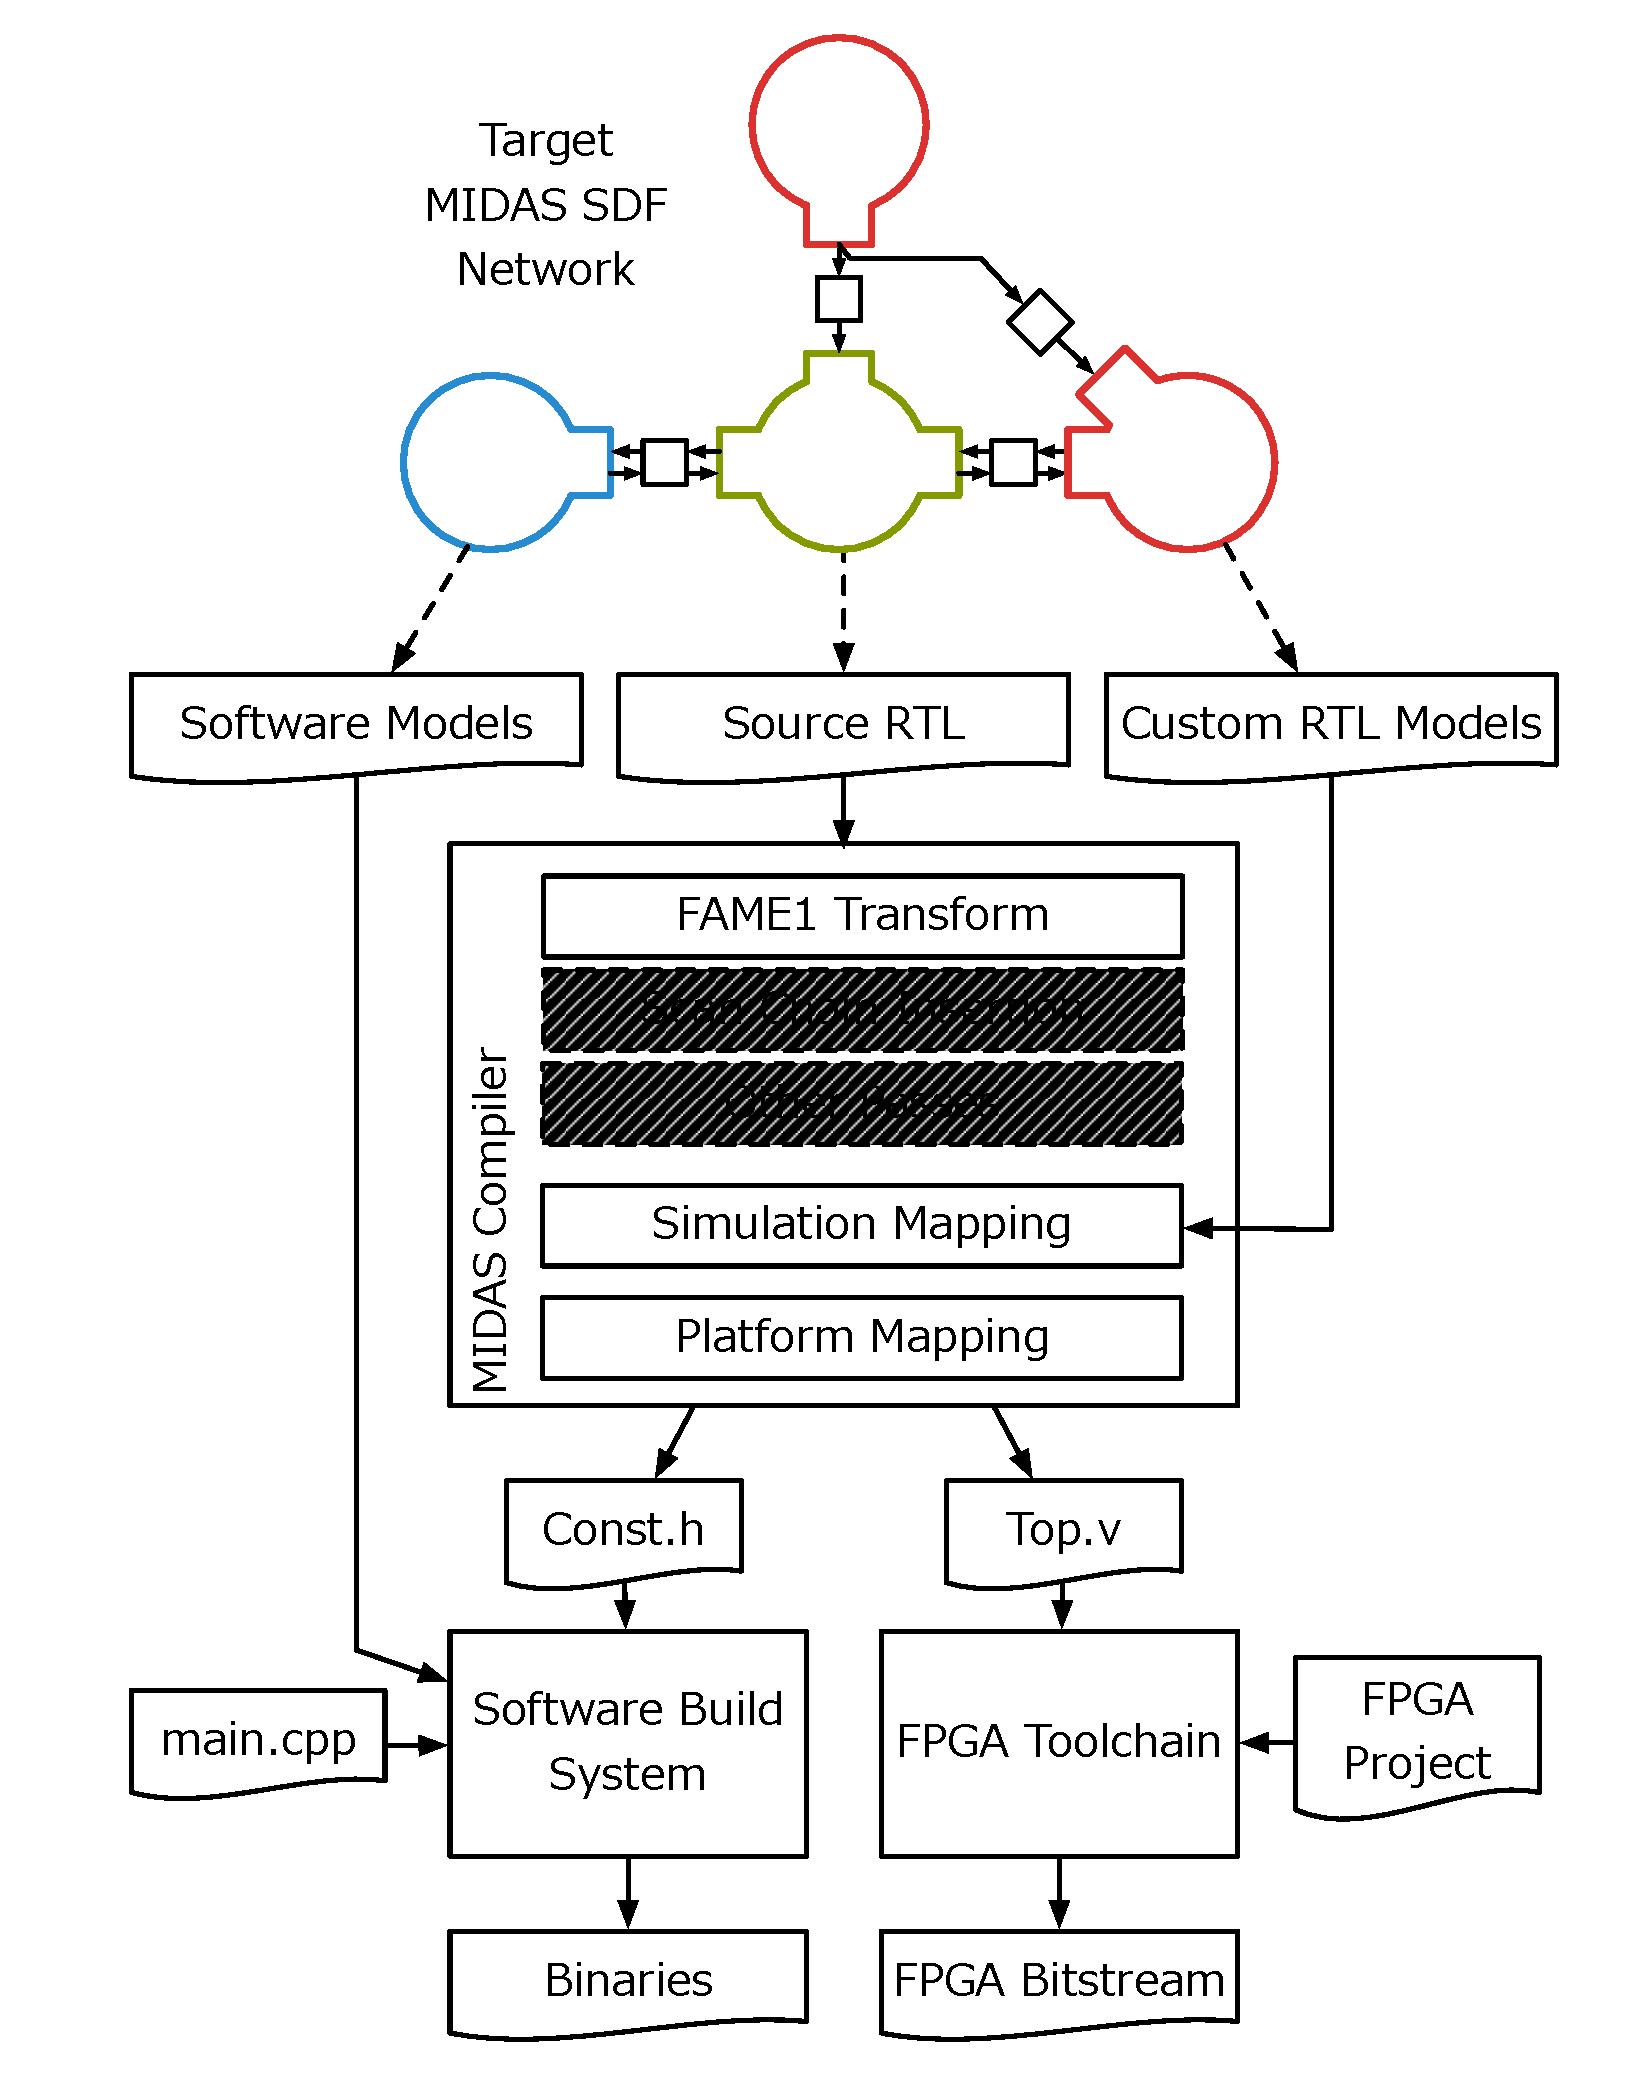
\includegraphics[width=16cm]{figures/toolchain.pdf}
	\caption{An overview of the MIDAS flow.  }
	\label{fig:midas}
\end{figure}

MIDAS is a set of C++ and RTL libraries alongside a compiler. The current MIDAS
flow is shown in figure \ref{fig:midas}. MIDAS accepts a description of target
as a synchronous dataflow-like network of interconnected models, which
specifies how it is composed of source RTL, software models, and custom RTL
models. The MIDAS compiler then automatically transforms source RTL into
host-decoupled RTL models, instrumenting them if desired. MIDAS then performs a
\emph{simulation mapping}, during which transformed models are connected to
custom RTL models with \emph{channels} and to off-fabric models with
\textit{channel endpoints} that implement latency-insensitive communication
between models on different parts of the host-platform. During this process,
the compiler builds up a memory map of all the simulation constituents and
generates a simulation interconnect. In \emph{platform mapping}, the
simulation-mapped design is connected to the memory and communication resources
exposed by the FPGA-host. The compiler emits a verilog file that is compiled
into a FPGA project to produce a simulator bitstream and the simulation memory
map.

With this memory map, the simulation designer defines a \emph{master} program,
which links in software models that constitute the remainder of the target, and
sequences simulation by invoking commands defined in the MIDAS API. These
commands are implemented as MMIO made over the generated simulation
interconnect.

\section{Target Specification and Simulation Abstractions}\label{sec:sdf}

In MIDAS, the target design is specified as a synchronous dataflow-like (SDF)
network of \emph{models}, connected with FIFO \emph{channels}, that carry
simulation \emph{tokens}(this is akin to model of computation presented
RAMP\cite{ramp} and APorts\cite{APortNetworks}). This description is sufficient
to capture the RTL behavior of the target, while still enabling a wide range of
optimizations that make FPGAs more effective accelerators for simulation.  A
illustration of an SDF describing a 32-bit unsigned adder is shown in figure
\ref{adder-example}.

\begin{figure}
	\centering
	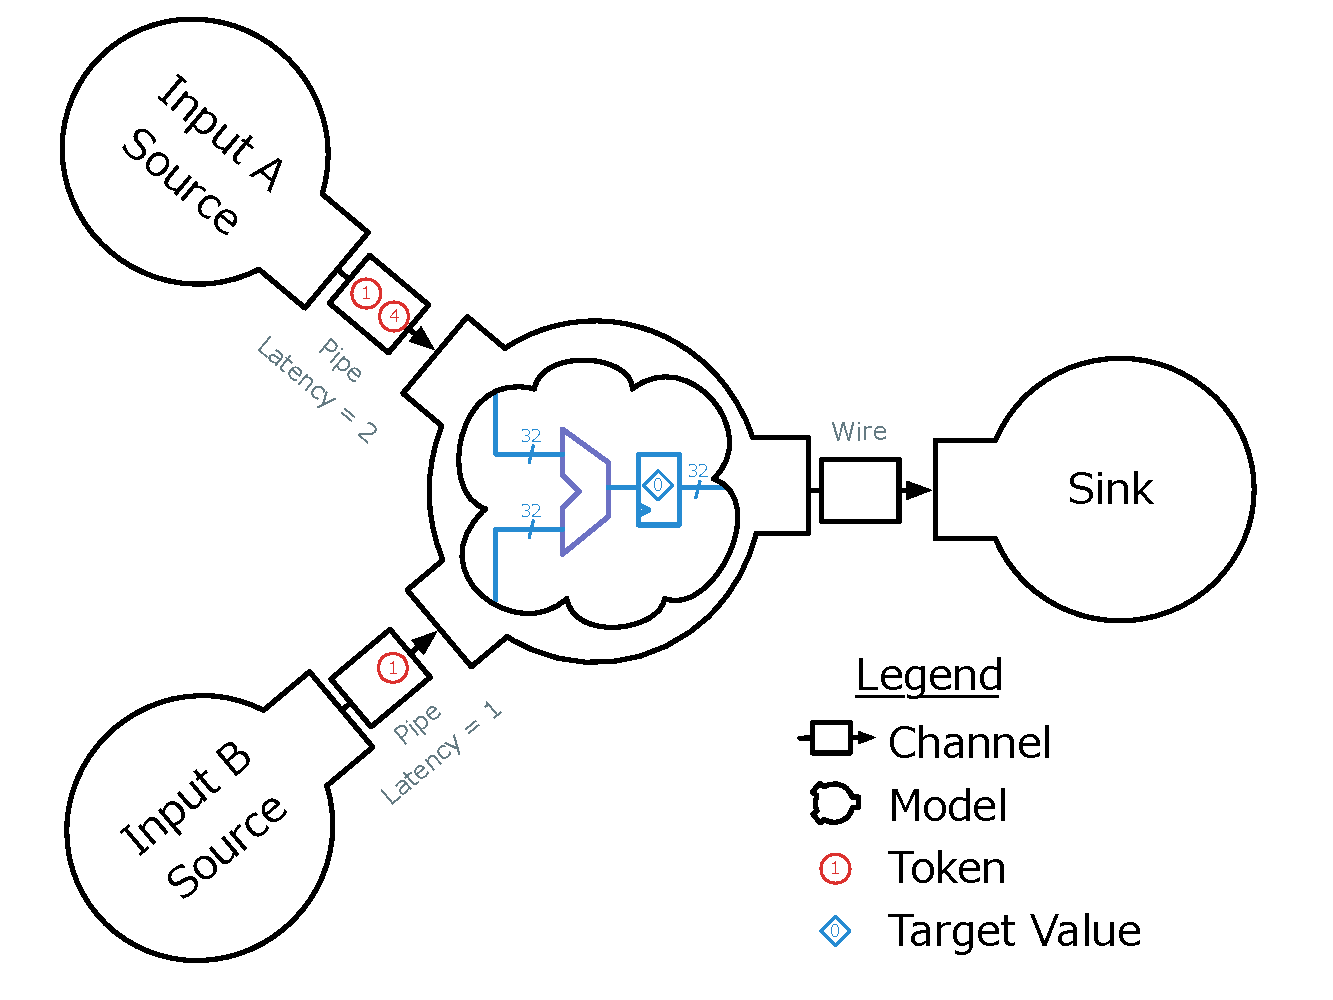
\includegraphics[width=16cm]{figures/adder-example.pdf}
    \caption{A MIDAS SDF description of a 32-bit unsigned adder with latency of
    one, and the tokens as they would be initialized at time 0.}
	\label{fig:adder-example}
\end{figure}

\emph{Models} capture the behavior of a synchronous block of digital logic (an
ALU, a processor pipeline, a cache, etc...). A model advances one cycle in
target time, by dequeuing a single token from each of its input channels, and
has enqueuing a single token into each of its output channels.  Models must
dequeue from each input and into enqueue each output exactly once before they
may dequeue younger inputs: they may never ``peek" at younger tokens.

\emph{Tokens} are the basic quantum of data in the simulation. A token is
defined by a type, which corresponds to the target wire that carries it, and
value on that wire after it has ``settled" for that cycle (more on this later).

\emph{Channels} carry tokens between model in FIFO order, and simulate the
target interconnect between those models. There is a single primitive type of
channel --  the \emph{pipe} -- which represents a wire with 0 or more
registers. Pipes may also implement clock domain crossing (CDC) by duplicating
or destroying tokens based on the relative clock frequency of the two models.
\footnote{The channel differs from a classical SDF channel in two ways.
Firstly, to implement CDC in an SDF, an intermediate process would need to be
placed between two channels. Second, MIDAS channels are not infinitely deep.
(Though, one could mimic a finite channel in an SDF with a bidirectional pair
of channels: one carrying the original tokens from source to sink, and the
second carrying credit tokens from sink to source. This is effecively what
happens in MIDAS, as models must check there output queues are not full
(equivalent to consuming a credit token) before firing.)} To describe latency
insensitive interconnect in a target, MIDAS also exposes a \emph{queue} type
channel. Using queue-type channels permits simulation optimizations that would
be impossible by describing the same interconnect with some combination of
pipes and models.

At time zero each of the channels is intialized with a sequence of tokens based
on the type of target interconnect they model.  A pipe is intialized with
tokens equal to its latency. Thus, a channel that models a wire is intialized
with zero input tokens. After initialization, target time advances in a
decoupled fashion with models firing whenever their tokens becomes available
and their output channels have space. The figures \ref{fig:adder-execution}a -
\ref{fig:adder-execution}d illustrate the this with the example SDF in figure
\ref{fig:adder-example} over two target cycles.

\begin{sidewaysfigure}
    \begin{subfigure}[t]{0.45\textwidth}
	    \centering
        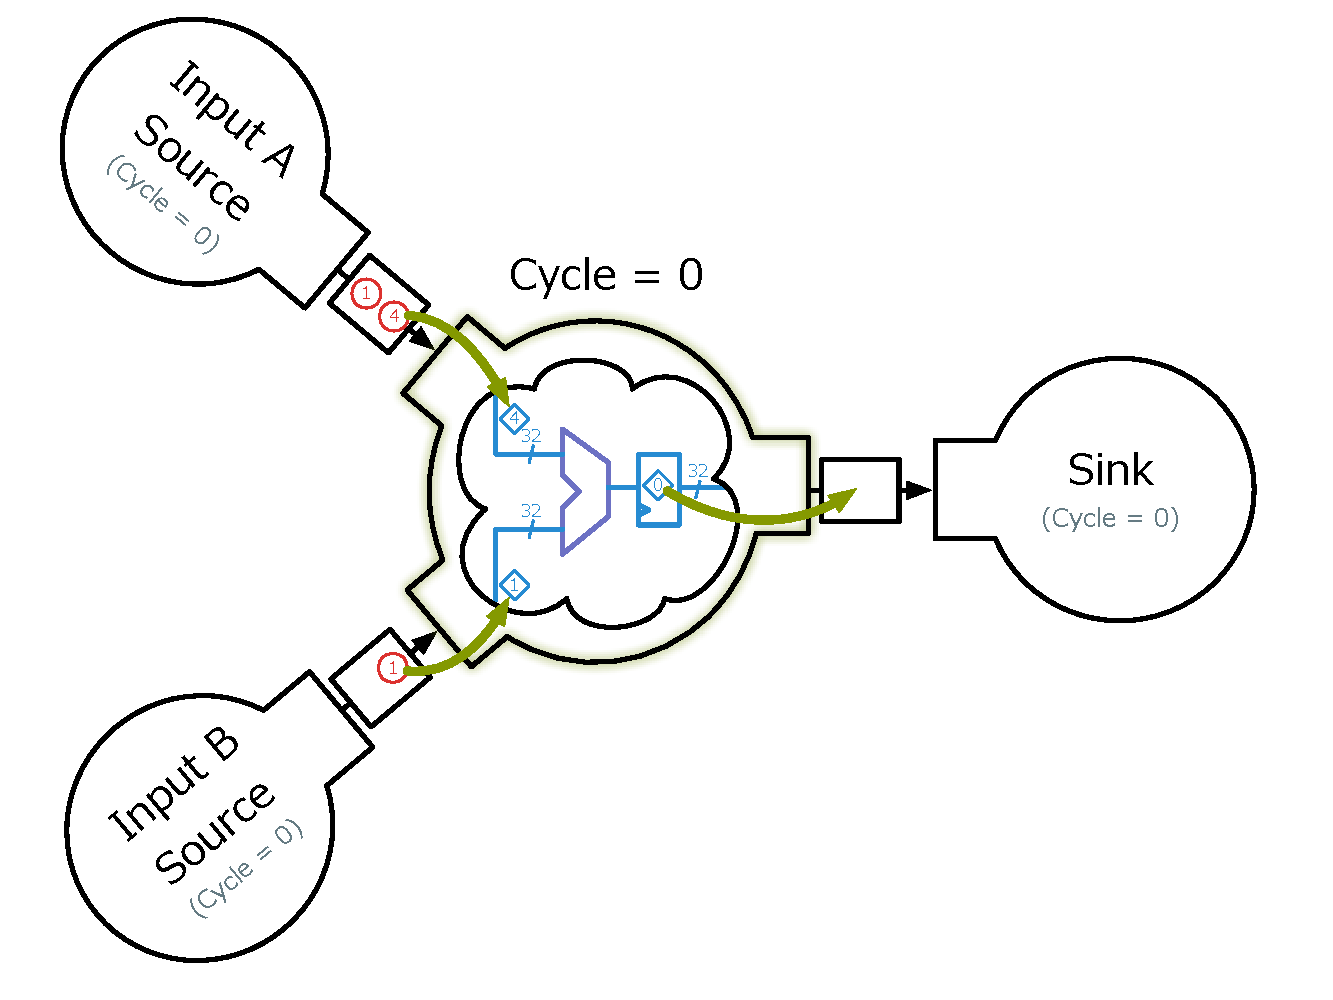
\includegraphics[width=\linewidth]{figures/adder-ex1.pdf}
        \caption{The adder fires cycle 0, advancing ahead of the other models
        in the graph.}
    \end{subfigure}
    \begin{subfigure}[t]{0.45\textwidth}
	    \centering
        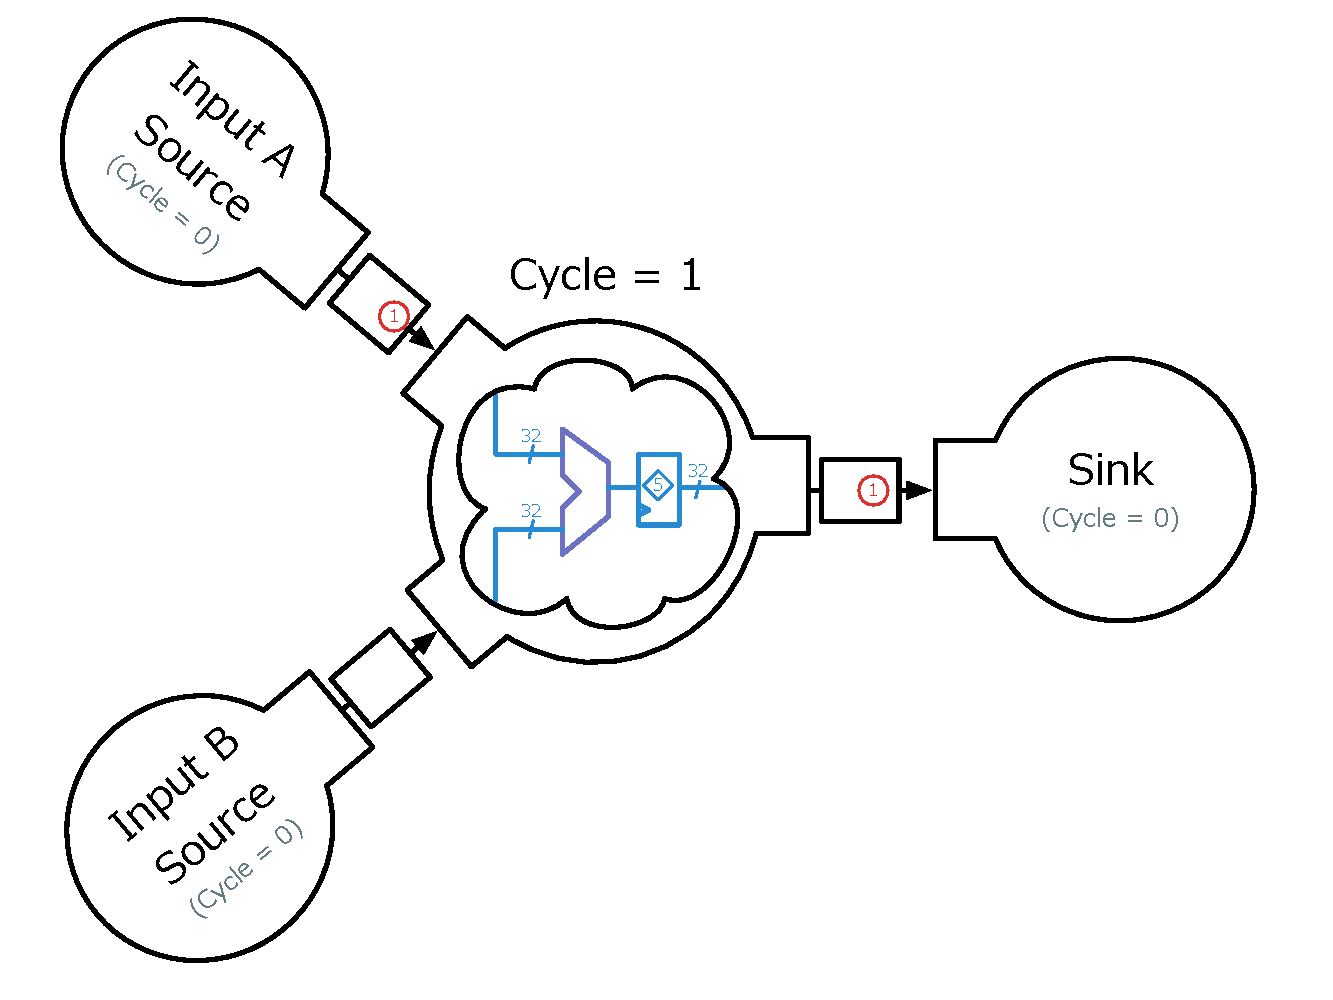
\includegraphics[width=\linewidth]{figures/adder-ex2.pdf}
        \caption{Having advanced to the next cycle, the adder model stalls as
        it cannot proceed until there is another B input token}
    \end{subfigure}
    \begin{subfigure}[t]{0.45\textwidth}
	    \centering
        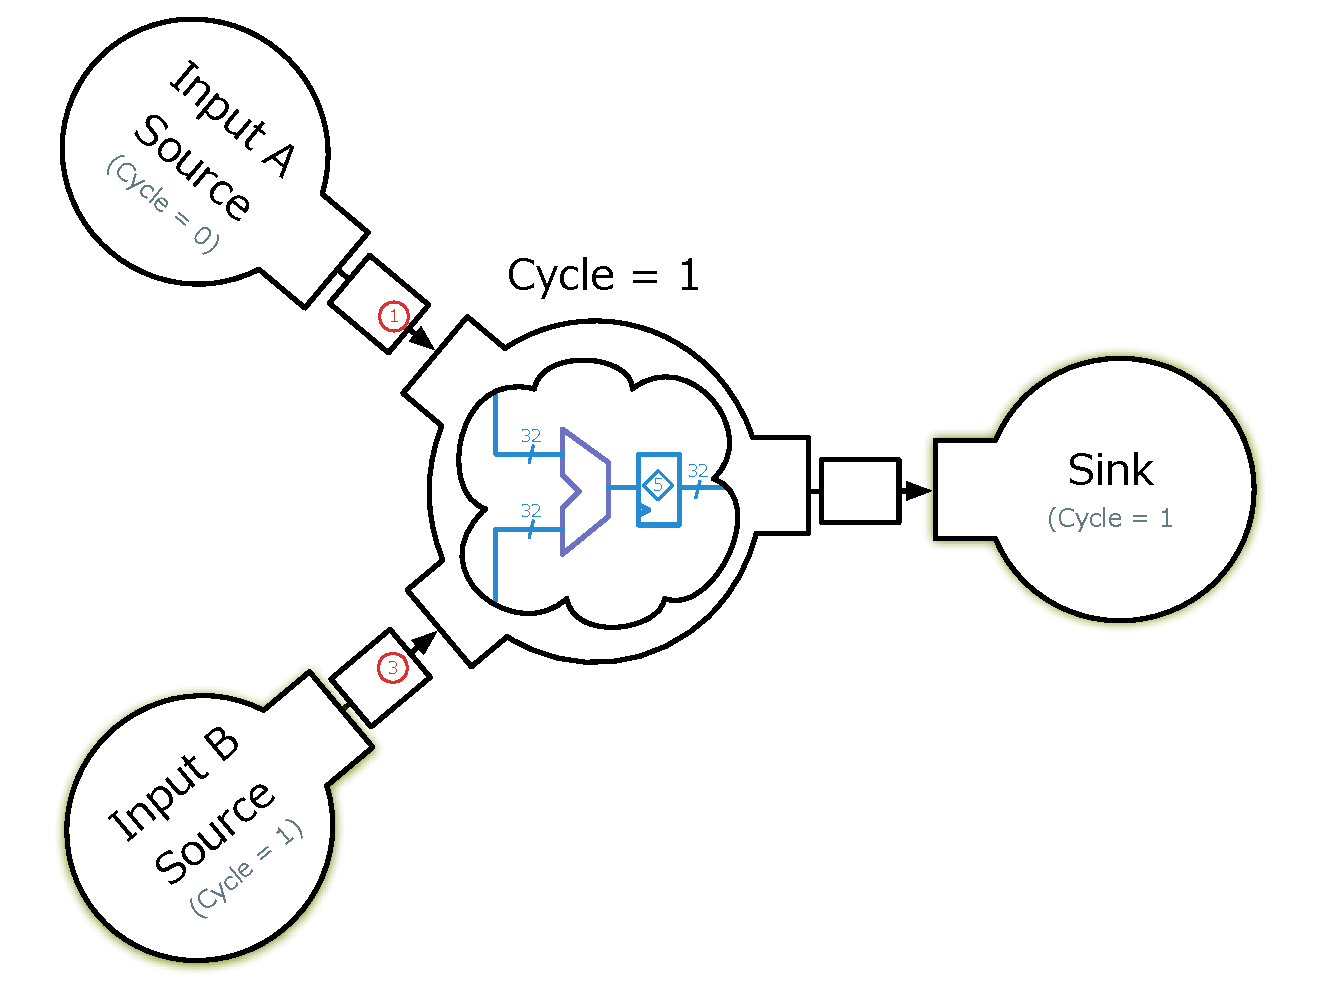
\includegraphics[width=\linewidth]{figures/adder-ex3.pdf}
        \caption{Eventually, input B model fires providing the needed token. The sink may or
        may not have consumed the output in this time.}
    \end{subfigure}\hspace{0.1\linewidth}
    \begin{subfigure}[t]{0.45\textwidth}
	    \centering
        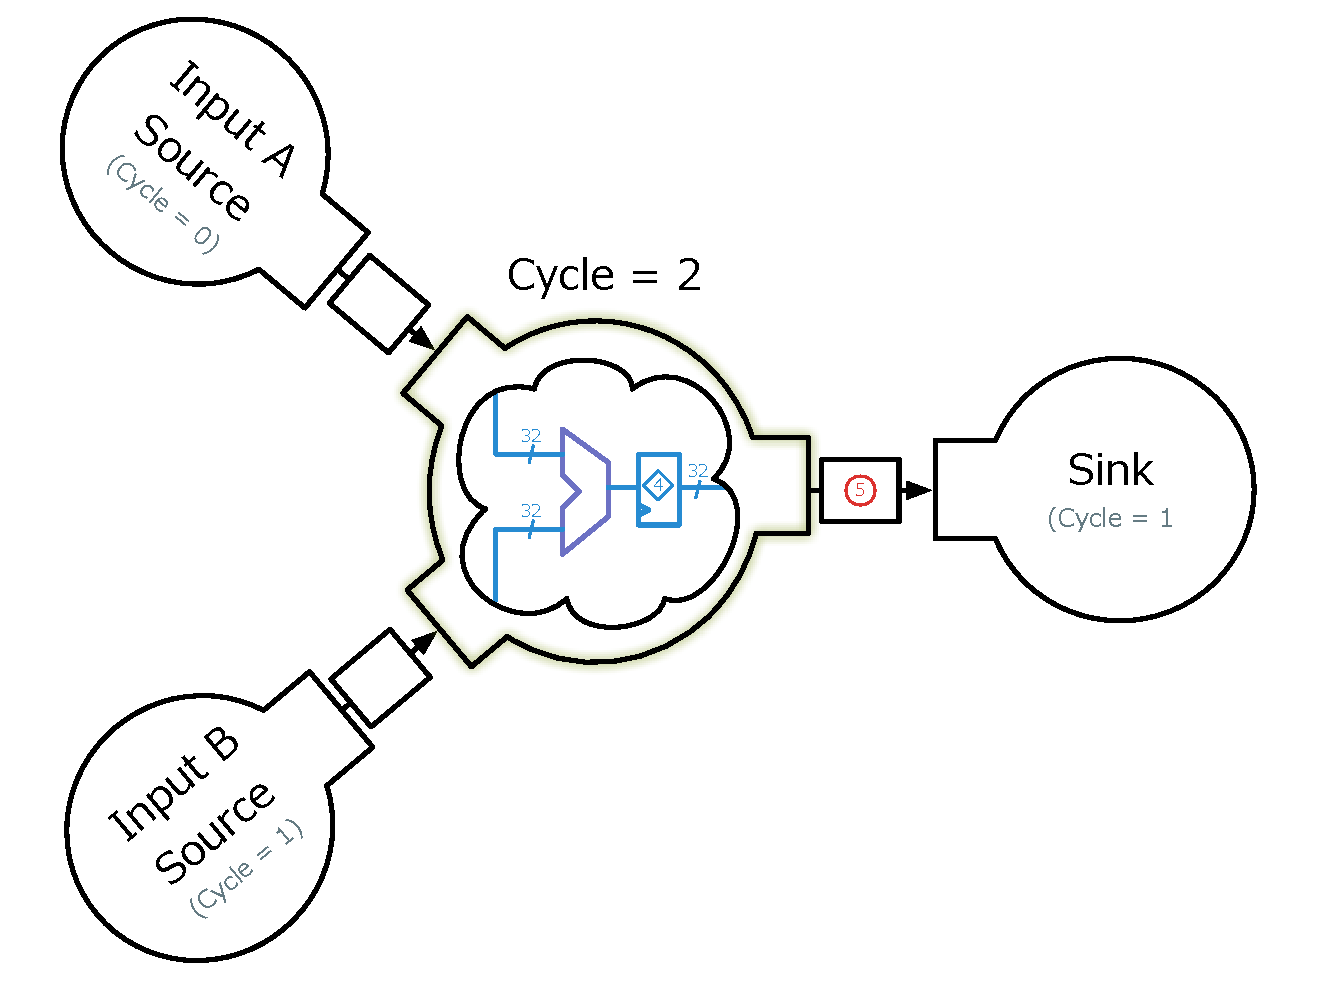
\includegraphics[width=\linewidth]{figures/adder-ex4.pdf}
        \caption{The state of the graph after the model fires a second time.}
    \end{subfigure}
    \caption{Example execution of the adder SDF advancing two target cycles.}
    \label{fig:adder-execution}
\end{sidewaysfigure}

\emph{Deadlock} occurs if no model can advance (not all of its inputs are
valid, or it's outputs are not ready to accept a new token). Generally, this
occurs when the SDF includes a combinational path that passes through zero or
more other models before feeding back into itself -- it need not be a
combinational loop. \TODO{This is demonstrated in example K.} Judicious choice
of channel type (for instance using queues or pipes with non-zero latency) is
required to prevent this.

A simulation that faithfully implements an SDF of this form decouples
target time from host time: it may take an arbitrary (but finite) host time for
tokens to pass through channels, or for models to fire.  Moreover, the
simulation may optimized automatically by performing transformations on models
that maintain their token input-output behavior.

When a model is hosted on an FPGA this implies that one target cycle may
execute over an arbitrary number of FPGA-host clock cycles.  ASIC structures
that map poorly to an FPGA when implemented directly, like CAMs and
multi-ported RAMs, can instead by simulated over multiple host cycles with
fewer resources and greater host frequency.

To help quantify this time-area trade off it is useful to define FPGA-cycle to
Model-Cycle Ratio\cite{APorts}: $$ FMR = \frac{Cycles_{FPGA}}{Cycles_{Target}}
$$

\noindent The rate at which the model simulates is thus given by:

$$ f_{model} = \frac{f_{FPGA}}{FMR} $$

\section{The MIDAS Compiler Flow}

\subsection{Source Tranformations}\label{sec:source-transformations}

Source RTL must be transformed to conform to MIDAS' SDF model of computation.
To do this, MIDAS uses a FIRRTL compiler pass that adds an additional enable,
\emph{target-fire}, to all target registers and to the write ports of
sequential memories. A model generated in this way can achieve an FMR of 1,
assuming its input tokens are always available and its output queues are never
full.  However, this model is FPGA resource inefficient as it is implementing
the RTL directly (like an FPGA prototype), and introduces a high fan-out net in
target-fire that may adversely affect cycle time for sufficient large blocks of
RTL.

Additional transformations may be invoked to add scan chains and I/O trace
buffers for debugging, and for state snapshotting for use with
Strober\cite{strober}. See figure \ref{fig:midas-passes}.

\begin{figure}
	\centering
	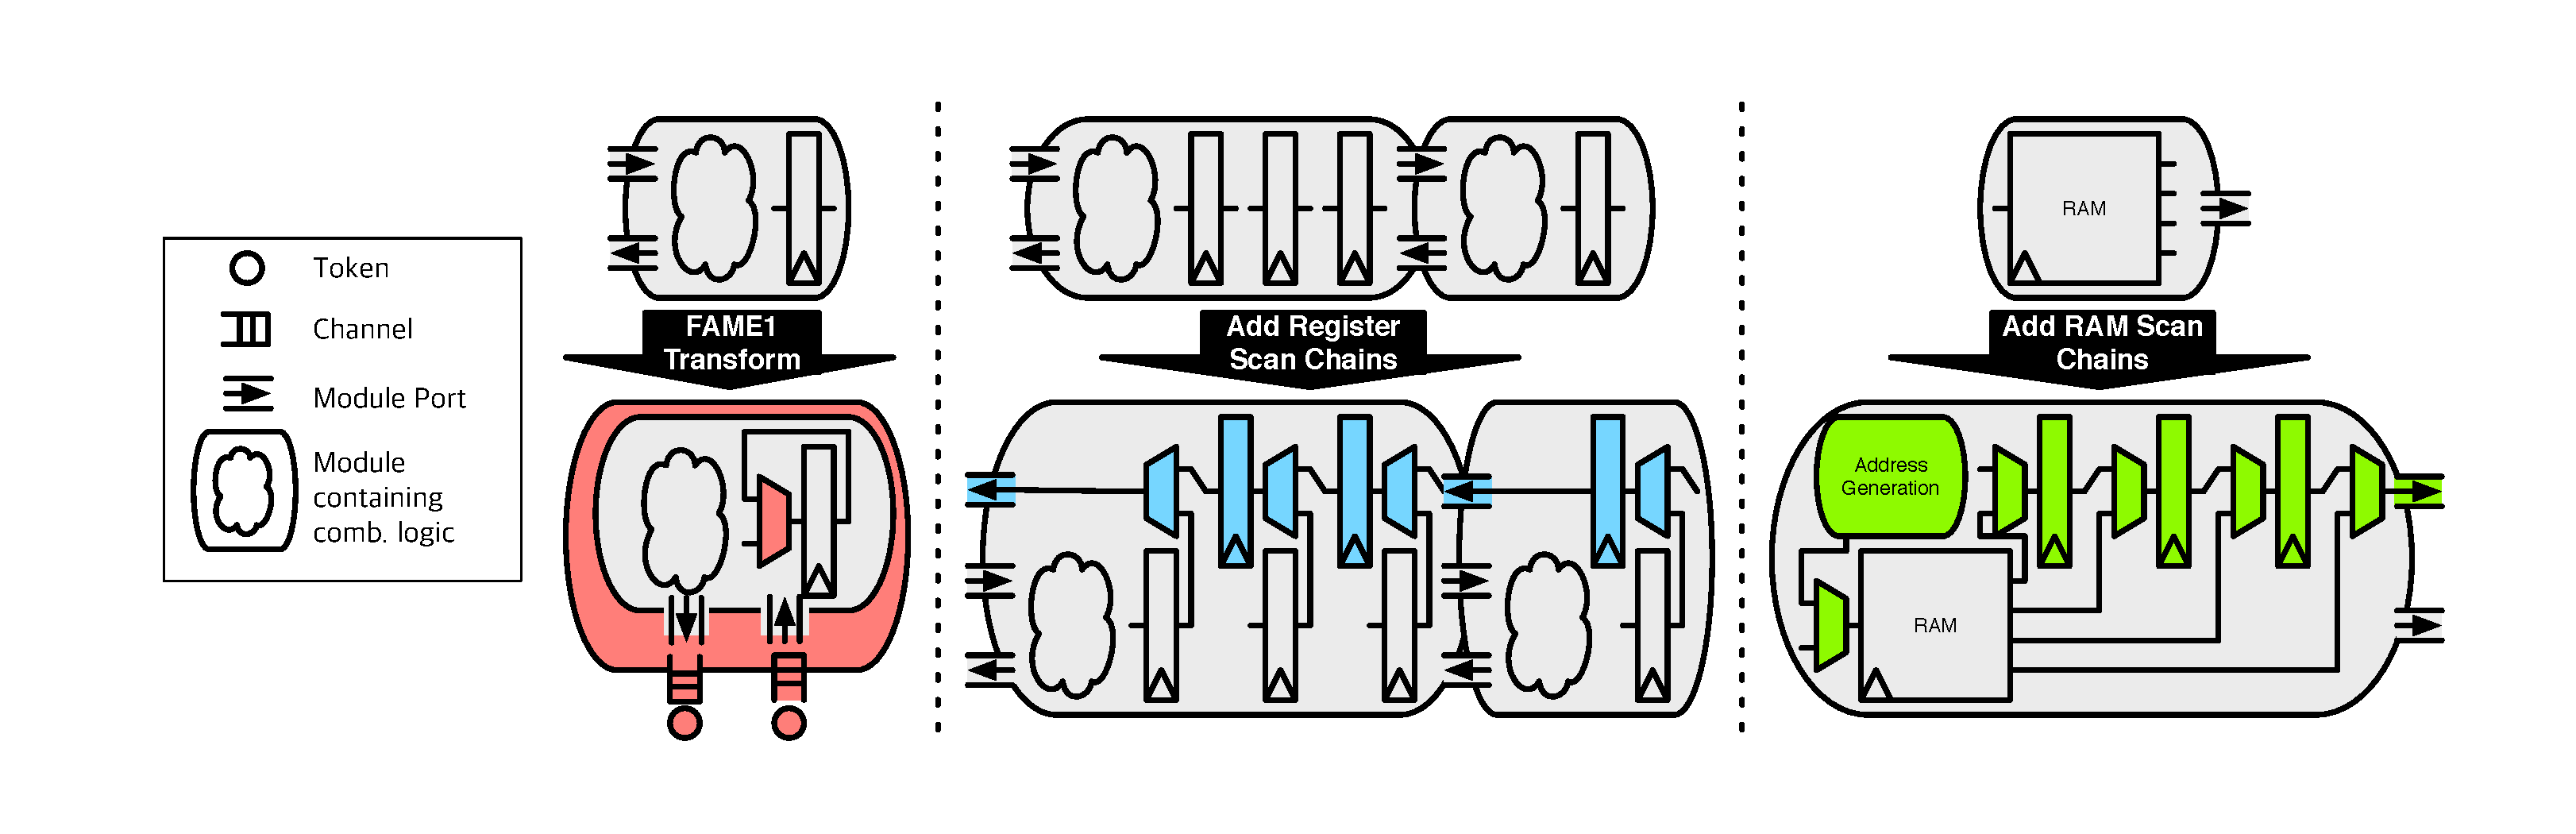
\includegraphics[width=16cm]{figures/midas-passes.pdf}
	\caption{Passes supported by MIDAS required for Strober energy measurements.}
	\label{fig:midas-passes}
	\centering
\end{figure}

\subsection{Simulation Mapping}

Once source RTL has been transformed into models, MIDAS generates a
host-agnostic simulation mapping of the SDF. Using Chisel3, MIDAS generates
simulation queues that implement the channels of the SDF. If a channel would
cross over the boundary of the local FPGA, MIDAS generates an \emph{endpoint},
a memory-mapped queue, whose sister endpoint resides on a different part of the
host platform.  Together, these endpoints implement a simulation channel.
Remaining I/O left unconnected on source-RTL models are bound to the default
I/O model, which act as an infinite source and/or sink of tokens.  When acting
as a source, the default I/O model emits tokens whose value set by a
memory-mapped register.

During this process, MIDAS also emits \emph{widgets}, memory-mapped modules
that provide simulation utilties but do not simulate target time (they are not
models). These widgets include scan chain and I/O trace buffer controllers, a
module used to initialize or dump FPGA-local DRAM, and a a controller, that can
reset simulation to time 0 and regulates the advance of target time on the
FPGA.

Once all of the simulation components (widgets, models, endpoints. etc...) have
been elaborated, the simulation interconnect is emitted and bound to an AXI4
slave port. All simulation memory-mapped components are managed with MMIO
through this interface. Similarly, components that require FPGA-local DRAM are
bound a single AXI4 master port.

\subsection{Platform Mapping}

In attempt to orthogonalize MIDAS from the complexities of FPGA toolchains,
MIDAS requires that each FPGA-host implement a skeleton project that exposes
standard interfaces to its periphery IP such as memory controllers for
FPGA-local DRAM, and communication IP, like PCI-E and ethernet controllers.
These projects must also expose a clock and synchronous reset which will drive
the MIDAS generated RTL.  During platform mapping, MIDAS bridges out the AXI-4
master and slave interfaces of the simulation-mapping to the interfaces
presented by the project.

Finally, MIDAS then emits a ``*Shim.v" that can be compiled into the
aforementioned FPGA project, and a C++ header ``*const.h" that describes the
memory map of simulator residing on that particular FPGA.

\section{MIDAS API \& Master Program}

To control the simulation, the user must define a master program, linking in
the MIDAS C++ libraries, the compiler-generated header and a simulation MMIO
driver.  The library implements primitive commands to control the simulation
such as \emph{step/advance K}, \emph{reset}(these commands will eventually
constitute the ``MIDAS API"). Each of these commands is implemented with
simulation MMIO.  Widgets, endpoints, and models instantiated in simulator have
their own drivers that extend the primitive commands.  For example, the default
I/O model has \emph{peek}, which reads the value of the last token sunk through
one of its ports, and \emph{poke}, to change the value of tokens it generates.  The
simulation driver, is host-platform specific and implements simulation MMIO by
tunneling requests to and from different parts of the host.

\section{Target \& Host Machines of this Report}\label{sec:targetandhostmachines}

While MIDAS has preliminary support for other host platforms, all the
experiments of this report are run on Xilinx ZC706 development boards, which
feature a Zynq XC7Z045 FPGA. These FPGAs have a processing system (PS),
consisting of hardened ARM A9 with 512 MiB of DRAM connected to the
programmable logic(PL), which implements the Kintex-7 fabric architecture with
19.1Mb of BRAM and 350K logic cells. The PS is connected to the PL though a
number of interfaces, including 4 general purpose 32-bit AXI-4 master ports.
Linux processes running on the PS interact with the PL with MMIO over this
interfaceFinally, the PL is connected to a configurable DDR PHY, which on the
ZC706, drives a DDR3 SODIMM (8GiB).

All target designs used in this report are single-core, tethered RISCV
processors with a single-channel DRAM subsystem.  They all share the MIDAS SDF
shown in figure \ref{default-target}. This SDF has one transformed-RTL model
sourced from RocketChip that instanstiates the processor pipeline (Rocket or
BOOM) with L1 caches and uncore (which contains the TileLink agent that manages
the tether), a software model, that wraps the RISC-V front-end server
(\texttt{riscv-fesvr}) which facilitates tethered boot and to which console I/O
is proxied from the target, and the memory-timing model instance, which
connects a an AXI4 interface mastered by the processor. Whatever remaining I/O
coming off the transformed model, including reset, is bound to the default I/O
model.

\begin{figure}
	\centering
	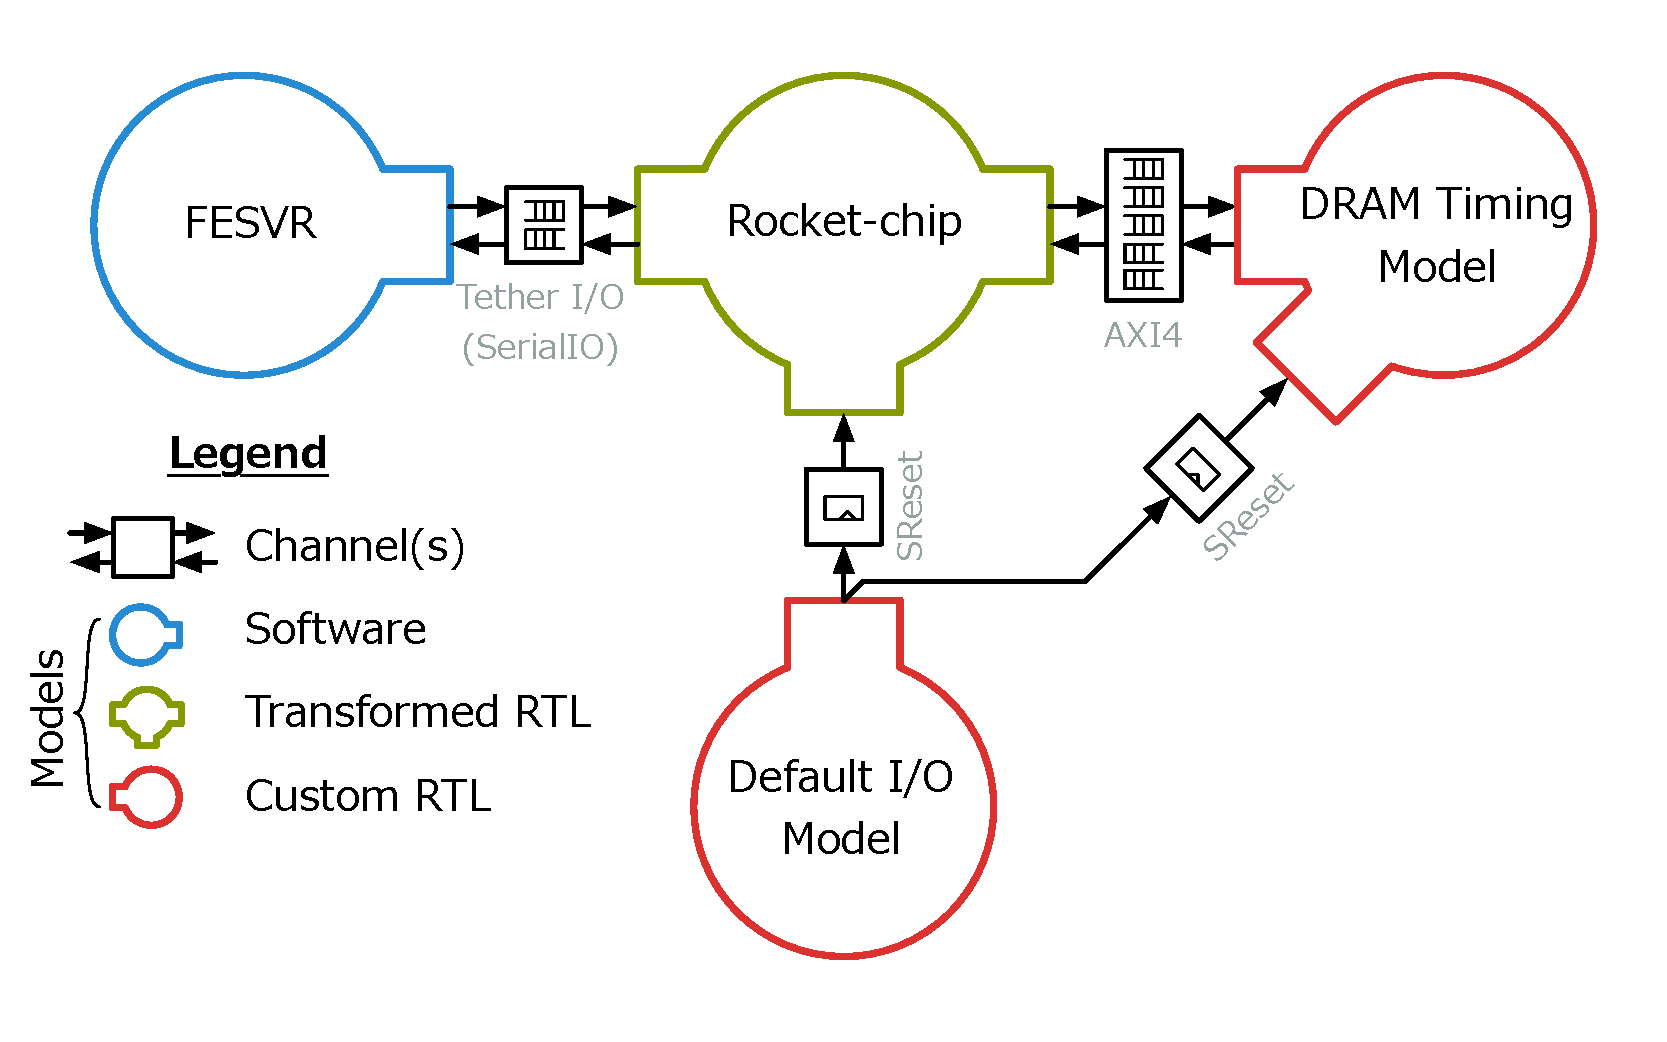
\includegraphics[width=16cm]{figures/masters-target.pdf}
    \caption{The MIDAS SDF of the target design used in this report. Channel
    details and initial tokens are omitted for simplicity. Both the tether I/O
    and AXI4 have bidirectional decoupled (ready-valid) target interconnect,
    thus the channels are impemented as sets of queues. SReset channels are pipes with
    a latency of one.}
	\label{fig:default-target}
\end{figure}

All targets are mapped to the ZC706 with the master program and
\texttt{riscv-fesvr} software model hosted on the PS (running in a single linux
process) while the transformed RTL and memory-timing model are hosted in the
PL. The AXI4 slave interface of the simulation-mapped design is bound to the 32
bit AXI4-GP0 master; the simulation MMIO driver simply mmaps the memory region
bound to that port into the process' memory space.  The AXI4 master presented
by the simulation mapping is bound directly to the slave interface presented by
the DDR3 controller of the PL. See figure \TODO{Da figure!}
